\documentclass[12pt,reqno]{amsart}



\setcounter{tocdepth}{2} %%profundidade da numeracao no sumario
\setcounter{secnumdepth}{4}

\usepackage{psfrag}
\usepackage{graphicx}
\usepackage[english,brazil]{babel}
\usepackage[utf8]{inputenc}
\usepackage{textcomp}
\usepackage[T1]{fontenc}
\usepackage{lmodern}
\usepackage{fullpage}
\usepackage{pdfpages}
\usepackage[margin=10pt,labelfont=bf]{caption}

%----------------------------
\usepackage{eurosym}

\usepackage{color}
\usepackage{geometry}
%
\geometry{left=25mm,right=25mm, top=25mm, bottom=30mm}

%\usepackage[colorlinks,backref]{hyperref}
\usepackage[]{hyperref}
\usepackage{srcltx}
\usepackage{multicol}
\usepackage{array}
\usepackage{enumerate}   
\usepackage{amssymb}

\usepackage{mathtools} %%symbols as :=
\usepackage{tikz} %% permite tikz
\usepackage{svg}    %%ibagens
\usepackage{ragged2e} 					%%added provides \RaggedLeft


%\setcounter{page}{-2}

\makeatletter
\renewcommand{\labelenumi}{\theenumi.}
\makeatother

%%%%%%%%%%%%%%%%%%%%%%%%%%%%%%%%%%%%%%%%%%%%%%%%%%%%%%%%%%%%%%%%%%%%%%
\let\epsilon\varepsilon
%%%%%%%%%%%%%%%%%%%%%%%%%%%%%%%%%%%%%%%%%%%%%%%%%%%%%%%%%%%%%%%%%%%%%%

\newtheoremstyle{note}% name
  {3pt}%      Space above
  {4pt}%      Space below 
  {\sl}%      Body font
  {}%         Indent amount (empty = no indent, \parindent = para indent)
  {\bfseries}% Thm head font
  {.}%        Punctuation after thm head
  {.5em}%     Space after thm head: " " = normal interword space;
                                %       \newline = linebreak
  {}%         Thm head spec (can be left empty, meaning `normal')

  
  
\def\tand{\ \text{and}\ }
\def\qand{\quad\text{and}\quad}
\def\qqand{\qquad\text{and}\qquad}

\let\emptyset=\varnothing
\let\setminus=\smallsetminus
\let\backslash=\smallsetminus
\let\subset\subseteq
\let\log=\ln

\newcommand{\K}{K_{\ell,r}} %%add by Paulo

\newcommand\cca{{\mathcal{A}}}
\newcommand\ccc{{\mathcal{C}}}
\newcommand\ccd{{\mathcal{D}}}
\newcommand\ccg{{\mathcal{G}}}
\newcommand\ccf{{\mathcal{F}}}
\newcommand\cch{{\mathcal{H}}}
\newcommand\cck{{\mathcal{K}}}
\newcommand\ccl{{\mathcal{L}}}
\newcommand\ccn{{\mathcal{N}}}
\newcommand\ccp{{\mathcal{P}}}
\newcommand\ccr{{\mathcal{R}}}
\newcommand\cct{{\mathcal{T}}}
\newcommand\ccq{{\mathcal{Q}}}
\newcommand\ccv{{\mathcal{V}}}
\newcommand\ccw{{\mathcal{W}}}
\newcommand\bbn{{\mathds{N}}}
\newcommand\abs{\mathop{\textrm{\rm abs}}\nolimits}
\newcommand\res{\mathop{\textrm{\rm res}}\nolimits}
%\newcommand\til{\mathop{\textrm{\rm til}}\nolimits}
\newcommand\cte{\mathop{\textrm{\rm cte}}\nolimits}
\newcommand\ini{\mathop{\textrm{\rm ini}}\nolimits}
\newcommand\out{\mathop{\textrm{\rm out}}\nolimits}

\let\phi=\varphi

\newcommand{\Phibad}{\Phi_{\textsc{bad}}}
%\homit make ``hom'' italic in definitions, lemmas and theorems.
\newcommand{\homit}{{\textrm{hom}}}
\newcommand{\opp}{{\textrm{opp}}}
\newcommand{\colour}{{\textrm{colour}}}

\def\til{\tilde}


\def\NN{\mathds N}
\def\ZZ{\mathds Z} 
\def\QQ{\mathds Q}
\def\RR{\mathds R}
\def\PP{\mathds P}
\def\EE{\mathds E}

\def\cB{\mathcal B}
\def\cR{\mathcal R}

\def\ra{\longrightarrow}
\def\red{\text{\rm red}}
\def\blue{\text{\rm blue}}
\def\R{\text{\rm red}}
\def\B{\text{\rm blue}}

\def\T{{\mathcal T}}



\def\mcarrow{\xrightarrow[]{\raisebox{0.0mm}[0mm]{$\scriptstyle \rm mr$}}}

\def\rbarrow{\xrightarrow[]{\raisebox{0.0mm}[0mm]{$\scriptstyle \rm rb$}}}
\newcommand{\rb}{\xrightarrow{\text{\rm rb}}}


\let\eps=\varepsilon
\let\theta=\vartheta
\let\rho=\varrho
\let\phi=\varphi


\let\epsilon\varepsilon
\let\:\colon
\let\subset\subseteq
\let\supset\supseteq

\let\<\langle
\let\>\rangle
\def\llfloor{\left\lfloor}
\def\rrfloor{\right\rfloor}
\def\llceil{\left\lceil}
\def\rrceil{\right\rceil}
\let\ot\leftarrow
\def\set{^{\{\}}}

\def\pmc#1{p^{\rm rb}_{#1}}

\newtheorem{teorema}{Teorema}[section]       
\newtheorem{Afirmativa}[teorema] {Afirmativa}         
\newtheorem{lema}      [teorema] {Lema}         
\newtheorem{corolario} [teorema] {Corolário}     
\newtheorem{proposicao} [teorema] {Proposição}     
\newtheorem{fato}      [teorema] {Fato}          
\newtheorem{conjectura}[teorema] {Conjectura}    
\newtheorem{problema}  [teorema] {Problema}       
\newtheorem{questao}[teorema] {Questão}    
\newtheorem{aff}[teorema]{Afirmação}
\newtheorem{obs}[teorema]{Observação}


\theoremstyle{note}
\newtheorem{propriedade}  [teorema] {Propriedade}       
\newtheorem{defi}  [teorema] {Definição}       
\newtheorem{exercicio}  [teorema] {Exercício}       


\def\bba{{\mathbb A}}
\def\bbb{{\mathbb B}}
\def\bbc{{\mathbb C}}
\def\bbd{{\mathbb D}}
\def\bbe{{\mathbb E}}
\def\bbf{{\mathbb F}}
\def\bbg{{\mathbb G}}
\def\bbh{{\mathbb H}}
\def\bbi{{\mathbb I}}
\def\bbj{{\mathbb J}}
\def\bbk{{\mathbb K}}
\def\bbl{{\mathbb L}}
\def\bbm{{\mathbb M}}
\def\bbn{{\mathbb N}}
\def\bbo{{\mathbb O}}
\def\bbp{{\mathbb P}}
\def\bbq{{\mathbb Q}}
\def\bbr{{\mathbb R}}
\def\bbs{{\mathbb S}}
\def\bbt{{\mathbb T}}
\def\bbu{{\mathbb U}}
\def\bbv{{\mathbb V}}
\def\bbw{{\mathbb W}}
\def\bbx{{\mathbb X}}
\def\bby{{\mathbb Y}}
\def\bbz{{\mathbb Z}}

\def\cala{{\mathcal A}}
\def\calb{{\mathcal B}}
\def\calc{{\mathcal C}}
\def\cald{{\mathcal D}}
\def\cale{{\mathcal E}}
\def\calf{{\mathcal F}}
\def\calg{{\mathcal G}}
\def\hh{{\mathcal H}}
\def\cali{{\mathcal I}}
\def\calj{{\mathcal J}}
\def\calk{{\mathcal K}}
\def\call{{\mathcal L}}
\def\calm{{\mathcal M}}
\def\caln{{\mathcal N}}
\def\calo{{\mathcal O}}
\def\calp{{\mathcal P}}
\def\calq{{\mathcal Q}}
\def\calr{{\mathcal R}}
\def\cals{{\mathcal S}}
\def\calt{{\mathcal T}}
\def\calu{{\mathcal U}}
\def\calv{{\mathcal V}}
\def\calw{{\mathcal W}}
\def\calx{{\mathcal X}}
\def\caly{{\mathcal Y}}
\def\calz{{\mathcal Z}}



\def\PP{{\mathbb P}}
\def\EE{{\mathbb E}}
\def\ZZ{{\mathbb Z}}
\def\NN{{\mathbb N}}
\def\QQ{{\mathbb Q}}

\def\cP{{\mathcal P}}
\def\cL{{\mathcal L}}
\def\bfa{\textbf{a}}
\def\bfb{\textbf{b}}
\def\bfx{\textbf{x}}
\def\bfzero{\textbf{0}}

\def\ex{\mathop{\text{\rm ex}}\nolimits}
\def\exdeg{\mathop{\text{\rm exdeg}}\nolimits}
\def\circum{\mathop{\text{\rm circ}}\nolimits}
\def\PA{\mathop{\text{\rm PA}}\nolimits}
\def\posto{\mathop{\text{\rm posto}}\nolimits}
\def\ci{\mathop{\text{\rm ci}}\nolimits}
\def\BDD{\mathop{\text{\rm LMT}}\nolimits}
\def\TUPLE{\mathop{\text{\rm CG}}\nolimits}
\def\col{\mathop{\text{\rm col}}\nolimits}
\def\AR{\mathop{\text{\rm AR}}\nolimits}


\newcommand{\sr}{\hat{r}}
\def\bu{\mathop{\text{\rm bu}}\nolimits}

\newcommand{\orr}{\overrightarrow{r}} %%oriented size-ramsey symbols
\newcommand{\orq}{\overrightarrow{r_q}}


\makeatletter
\def\@setaddresses{\par
  \nobreak \begingroup
\footnotesize
  \def\author##1{\nobreak\addvspace\bigskipamount}%
  \def\\{\unskip, \ignorespaces}%
  \interlinepenalty\@M
  \def\address##1##2{\begingroup
    \par\addvspace\bigskipamount\indent
    \@ifnotempty{##1}{(\ignorespaces##1\unskip) }%
    {\scshape\ignorespaces##2}\par\endgroup}%
  \def\curraddr##1##2{\begingroup
    \@ifnotempty{##2}{\nobreak\indent{\itshape Current address}%
      \@ifnotempty{##1}{, \ignorespaces##1\unskip}\/:\ccpace
      ##2\par}\endgroup}%
  \def\email##1##2{\begingroup
    \@ifnotempty{##2}{\nobreak\indent{\itshape Endereços Eletrônicos}%
      \@ifnotempty{##1}{, \ignorespaces##1\unskip}\/:\ccpace
      \ttfamily##2\par}\endgroup}%
  \def\urladdr##1##2{\begingroup
    \@ifnotempty{##2}{\nobreak\indent{\itshape URL}%
      \@ifnotempty{##1}{, \ignorespaces##1\unskip}\/:\ccpace
      \ttfamily##2\par}\endgroup}%
  \addresses
  \endgroup
}
\makeatother

\def\({\left(}
\def\){\right)}  
\def\<{\langle}
\def\>{\rangle}
\let\:=\colon

\def\PP{{\mathbb P}}
\def\EE{{\mathbb E}}
\def\ZZ{{\mathbb Z}}
\def\NN{{\mathbb N}}
\def\QQ{{\mathbb Q}}

\def\cP{{\mathcal P}}
\def\cL{{\mathcal L}}
\def\bfa{\textbf{a}}
\def\bfb{\textbf{b}}
\def\bfx{\textbf{x}}
\def\bfzero{\textbf{0}}

\def\ex{\mathop{\text{\rm ex}}\nolimits}
\def\exdeg{\mathop{\text{\rm exdeg}}\nolimits}
\def\circum{\mathop{\text{\rm circ}}\nolimits}
\def\PA{\mathop{\text{\rm PA}}\nolimits}
\def\posto{\mathop{\text{\rm posto}}\nolimits}
\def\ci{\mathop{\text{\rm ci}}\nolimits}
\def\BDD{\mathop{\text{\rm LMT}}\nolimits}
\def\TUPLE{\mathop{\text{\rm CG}}\nolimits}
\def\col{\mathop{\text{\rm col}}\nolimits}

\newcommand{\etal}{\textsl{et al.}}

\usepackage{path}

\usepackage{setspace}
\onehalfspacing
\renewcommand{\baselinestretch}{1.2}

\begin{document}



\title[]{}

% \thanks{Instituto de Matem\'atica e Estat\'{\i}stica, Universidade de S\~ao
%   Paulo, Rua do Mat\~ao 1010, 05508--090~S\~ao Paulo, SP\\yoshi@ime.usp.br, mota@ime.usp.br}
%   
\maketitle
\thispagestyle{empty}
\begin{center}

\includegraphics[scale=0.3]{ufabc}\\
\vspace{.2cm}
\textbf{\Large UNIVERSIDADE FEDERAL DO ABC}\\
\vspace{.2cm}

{\sl TESE DE DOUTORADO\\ \ \\}
\end{center}

\begin{center}
{\bf PROBLEMAS DO TIPO RAMSEY E ANTI-RAMSEY EM GRAFOS DETERMINÍSTICOS E ALEATÓRIOS}\ \\ \
\end{center}

\indent{\bf Candidato:} Paulo Matias da Silva Junior\\
\indent{\bf Orientador:} Guilherme Oliveira Mota\\
\indent{\bf Instituição:} Universidade Federal do ABC -- UFABC

%\address{Centro de Matem\'atica, Computa\c c\~ao e Cogni\c c\~ao, Universidade Federal do ABC, Santo Andr\'e, Brazil}
%\email{g.mota@ufabc.edu.br, paulo.matias@aluno.ufabc.edu.br}

{\selectlanguage{brazil}
\begin{abstract}
  
  Este é o texto de defesa do doutorado e tem como foco o estudo de propriedades Ramsey 
  %%%xxxsize-Ramsey 
  e anti-Ramsey de grafos aleatórios e determinísticos.

Primeiro,
consideramos o problema proposto por Conlon e Tyomkyn, de determinar o menor número de cores necessárias para se colorir propriamente as arestas do grafo completo $K_n$,
de modo que nenhum par de triângulos vértices-disjuntos de $K_n$ tenham a mesma tripla de cores. 
Esta quantidade de cores era desconhecida para $n$ par e conseguimos computá-la para alguns casos pequenos e também para uma família infinita de valores de $n$.

Consideramos também o seguinte problema do tipo anti-Ramsey: dados grafos $G$ e $H$, denotamos por $G \rbarrow H$ a propriedade em que toda coloração própria de $E(G)$ apresenta uma cópia rainbow de $H$ em $G$.
Determinamos o valor da função limiar para $G(n,p) \rbarrow K_{\ell,r}$, para grafos bipartidos completos $K_{\ell,r}$ com $\ell,r \geq 3$.

%%%%xxxx Por último, o número de size-Ramsey de um grafo $H$ é o menor inteiro $m$ para o qual existe um grafo $G$ com $m$ arestas tal que em toda 2-coloração de $E(G)$, há uma cópia monocromática de $H$. Na variante do número de size-Ramsey para grafos orientados, verificamos que inverter a orientação de uma única aresta de uma estrela orientada de $m$ arestas torna esse parâmetro quadrático.

\end{abstract}}

\newpage


\tableofcontents

\pagestyle{plain}
\footskip=20pt

\newpage

\section{Introdução}
\label{sec:intro}

Este trabalho de qualificação, elaborado pelo aluno de doutorado Paulo Matias da Silva Junior, no Centro de Matemática, Computação e Cognição, UFABC, enquadra-se na área de
combinatória extremal.

A Teoria de Ramsey é uma área da matemática que investiga a existência de ordem de subconjuntos dentro de conjuntos grandes de objetos.
O nome desse campo se deve ao resultado clássico de Frank P. Ramsey \cite{Ra} que provou que para quaisquer inteiros positivos $t$ e $q$, existe um inteiro $n$ tal que toda $q$-coloração do grafo completo $K_n$ contém uma cópia monocromática de $K_t$.

% Dentre as técnicas que pretendemos utilizar para atacar os problemas propostos, destacamos o Lema de Regularidade de Szemerédi e suas variantes (veja, por exemplo, \cite{gerke05:_sparse_survey, Kohayakawa97Szemeredi, KomlosSimonovits96, roedl05:PNAS, szemeredi76,  roedl10+:_graph_regul_lemmas, roedl07:_count,roedl07:_regul}). 

Dados grafos $G$ e $H$ e um inteiro positivo $q$, dizemos que $G$
\emph{é $q$-Ramsey para} $H$ se toda $q$-coloração das arestas de $G$ contém uma cópia monocromática de $H$.
Denotamos essa propriedade por $G\rightarrow (H)_q$.
Quando $q=2$, escrevemos simplesmente $G\rightarrow H$.
%Em sua forma mais simples, o clássico Teorema de Ramsey \cite{Ra} afirma que para qualquer grafo $H$ existe um inteiro $N$ tal que $K_N \rightarrow H$.
O \emph{número de Ramsey}~$r(H)$ de um grafo~$H$ é definido como o menor inteiro~$N$ com tal que $K_N \rightarrow H$.
Problemas em Teoria de Ramsey têm sido muito estudados e técnicas elegantes têm sido desenvolvidas  para estimar os números de Ramsey.
O trabalho de Conlon, Fox e Sudakov~\cite{CoFoSu15} contém um resumo  dos avanços na área.

%%% \text{\color{red} adicionar historia geral da area?}

%% \subsection{Organização do texto} \label{sec:justificativa}

Neste trabalho 
%% tem como objetivo o estudo de diversas propriedades de grafos que garantam a existência de estruturas monocromáticas e multicoloridas em grafos cujas arestas estão coloridas.
são investigadas propriedades do tipo Ramsey, anti-Ramsey
e size-Ramsey de grafos aleatórios e determinísticos em diferentes versões. 
%e problemas, o ponto em comum dos temas apresentados é a coloração de arestas. 

Iniciamos na Seção \ref{sec:triangles} com  um resultado de padrões em coloração de arestas do grafo completo. 
Especificamente, dado um natural $n$, calculamos a menor 
quantidade de cores em que existe uma coloração própria de $E(K_n)$ de modo a se evitar a formação de triângulos disjuntos em vértices que repetem a trinca de cores nas arestas.
Esse número era desconhecido quando $n$ é par e foi determinado para os primeiros números pares e para uma família infinita de valores de $n$.

%%%% seção conclusão?
%%%A importância e vigor da pesquisa em torno dos tópicos que propomos podem ser observados nos trabalhos clássicos de diversos pesquisadores renomados, como Erd\H{o}s, Rödl, Szemerédi, e Tao, dentre outros, e nos trabalhos modernos de proeminentes pesquisadores como Conlon, Gowers, e Schacht. 
%%% Os trabalhos desses autores, que muitas vezes consideram grafos aleatórios, mostram que ainda existe muito a ser feito no desenvolvimento de uma teoria sólida para entendermos a existência de uma certa ordem em estruturas aparentemente caóticas, o cerne da Teoria de Ramsey.

A propriedade anti-Ramsey estudada foi a de colorações próprias de arestas que contenham determinados subgrafos sem repetições de cores. 
 A Seção \ref{sec:anti} traz como resultado novo os detalhes para que essa propriedade ocorra em grafos aleatórios com relação a conter subgrafos  isomorfos ao grafo bipartido completo $\K$. 
A saber, dados os inteiros $r,\ell \geq 3$, provamos que o parâmetro de probabilidade para que um grafo aleatório possa ser colorido evitando cópias multicoloridas de $\K$ depende de uma relação com a densidade de $\K$.

%%%%xxxx O número size-Ramsey de um grafo $H$ é o menor número de arestas tal que existe um grafo $G$ com essa quantidade de arestas de modo que $G \rightarrow H$. A Seção \ref{sec:size} tem este número por tema, nela estudamos a literatura a respeito deste parâmetro para grafos simples,  hipergrafos e grafos orientados. 
%xxxxx Destacamos alguns resultados preliminares novos, especialmente de grafos orientados, em que calculamos os limitantes do número size-Ramsey para estrelas orientadas, mostrando que este número pode ser quadrático a depender da orientação escolhida para a estrela. Também exibimos o valor exato (ou um intervalo próximo) do número size-Ramsey  para grafos orientados pequenos com até $4$ vértices.




\section{Colorações próprias de arestas de grafos completos sem triângulos repetidos}
\label{sec:triangles}


%% Nesta seção \footnote{Os resultados descritos nesta seção foram desenvolvidos em um projeto conjunto com Fábio Botler, Lucas Colucci, Guilherme Mota, Roberto Parente e Matheus Secco.}, vamos considerar grafos finitos e simples. 
Os resultados descritos nesta seção foram desenvolvidos em um projeto conjunto com Fábio Botler, Lucas Colucci, Guilherme Mota, Roberto Parente e Matheus Secco.
Vamos considerar grafos finitos e simples. 
Recordamos que uma coloração de arestas é chamada de \emph{própria} se para cada par de arestas que compartilham um vértice em comum as cores são distintas. Um artigo recente de Conlon e Tyomkyn  \cite{conlontyomkyn} introduziu um novo conceito relacionado a colorações próprias, definido a seguir: 

\begin{defi}\label{def:fkn}
            Para $k,n\geq 2$ e fixado um grafo $H$, chamamos de $f_k(n,H)$ o menor inteiro $C$ tal que existe uma coloração
            própria de arestas de $K_n$ com $C$ cores sem conter $k$ cópias isomorfas em cores (\emph{repetições}) de $H$ disjuntas em vértices. 
\end{defi}


Para $H$ sendo um ciclo par, Conlon e Tyomkyn \cite{conlontyomkyn} perguntaram se para todo $\eps >0$,
existe um $t_0 = t_0(\eps)$ tal que, para todo 
$t \geq t_0$, $f_2(n, C_{2t}) = \Omega(2^{2-\eps})$.
%
Xu, Zhang, Jing e Ge \cite{ge2020color} provaram que $f_3(n, C_4) = \Theta(n)$ e depois refinaram a conjectura de Conlon e Tyomkym questionando se
$f_2(n, C_{2t}) = \Omega(n^{2-2/t})$. 
Por fim, Janzer \cite{janzer2020rainbow} resolve esse problema provando o seguinte resultado:
 
    \begin{teorema}\label{teo:janzer-ciclos}\cite{janzer2020rainbow}
           Sejam $k,t \geq 2$ inteiros fixados. Então $f_k(n,C_{2t}) = \Omega\big(n^{\frac{k}{k-1} \cdot\frac{t-1}{t}}\big)$.
    \end{teorema}

Nós estudamos o caso em que os parâmetros são $k = 2$ e $H = K_3$ na Definição \ref{def:fkn}. 
No artigo inicial de Conlon e Tyomkyn foi mostrado que $f_2(n,K_3) = n$ para
$n$ ímpar, e isso implica que $f_2(n,K_3) \leq n + 1$ para $n$ par. 
Além disso, como toda coloração própria de $K_n$ requer ao menos $n-1$ cores, segue que $f_2(n,K_3) \geq n- 1$.
Portanto, o problema que permanecera em aberto é decidir, para $n$ par, se $f_2(n,K_3)$ é igual a $n-1$, $n$ ou $n + 1$.

\subsection{Casos pequenos}

Nesta subseção, calculamos $f_2(n,K_3)$ para $n \in \{4,6,8,12\}$, o caso $n=10$ é coberto por um resultado apresentado na subseção seguinte. 
É evidente que $f_2(4,K_3) = 3$, dado que não existem pares de triângulos vértices-disjuntos em $K_4$, e com isso, busca-se simplesmente por qualquer coloração própria. 
Os próximos dois resultados mostram que, para $n = 6$ e $n = 8$, exatamente $n + 1$ cores são necessárias.

Chamamos dois triângulos vértices-disjuntos de \textit{similares} em uma coloração de um grafo se suas arestas recebem as mesmas três cores;  uma cor é dita ser \textit{cheia} se as arestas com tal cor formam um matching perfeito no grafo completo. 
Com essas breves definições podemos provar os resultados nos casos pequenos.

\begin{teorema}
       $f_2(6,K_3)=7$.
\end{teorema}
\begin{proof}
    Das considerações anteriores, é suficiente provar que 
    toda coloração de $K_6$ com no máximo seis cores contém um par de triângulos disjuntos em vértices que são \emph{similares} (i.e., triângulos cujas arestas recebem o mesmo conjunto de cores). 
   Suponha que isso não ocorre, e seja $V(K_6) =\{1,\dots,6\}$.
   Como $K_6$ tem $15$ arestas, e  cada uma dentre as seis classes de cor consiste de, no máximo, três arestas, tem-se que pelo menos três cores geram um emparelhamento perfeito (são cores \emph{cheias}). 
   Ademais, a união de quaisquer dois emparelhamentos perfeitos induzem um ciclo de comprimento seis.
   Supomos sem perda de generalidade que o ciclo $123456$ está colorido alternando as cores $1$ e $2$. 
   Nós chamamos uma aresta de \emph{corda curta} se ela conecta dois vértices com distância $2$ neste ciclo (em particular, uma corda curta forma um triângulo com arestas de cores $1$ e $2$). 
   É fácil ver que se temos três cordas curtas de mesma cor, então obtemos dois triângulos similares distintos. 
   Além disso, duas cordas curtas das mesmas cores devem ser da forma $i(i+2)$ e $(i+1)(i+3)$ para algum $i$ (índices mod $6$), já que de outra maneira elas gerariam dois triângulos disjuntos similares.
    
    Agora, suponha que existe alguma corda curta colorida com uma cor cheia, digamos que, a aresta $13$ está colorida com a cor $3$. É direto checar que as arestas restantes da cor $3$ devem ser $25$ e $46$, que é uma contradição, uma vez que $123$ e $456$ seriam triângulos similares.  
    
    Logo, nenhuma corda curta pertence a uma cor cheia. Como há $6$ cordas curtas e cada uma (de até três) cores que não são cheias pode cobrir, no máximo, duas cordas curtas, nós concluímos que toda cor que não é cheia aparece em exatamente duas cordas curtas. Sem perda de generalidade, supomos que $13$ e $24$ recebem a cor $4$, $35$ e $46$ a cor $5$, e $51$ e $62$ a cor $5$. Neste caso, os triângulos $135$ e $246$ são similares, o que é uma contradição.
\end{proof}


\begin{teorema}
     $f_2(8,K_3)=9$.
\end{teorema}
\begin{proof}
Pelas considerações anteriores, é suficiente provar que toda coloração do $K_8$ com no máximo $8$ cores  contém um par de triângulos similares disjuntos em vértices (i.e., triângulos cujas arestas recebem o mesmo conjunto de cores).
Suponha que não é esse o caso, e seja $\{1,\dots,8\}$ o conjunto de vértices do $K_8$. 
Como  $K_8$ tem $28$ arestas, e cada uma dentre as, no máximo, oito classes de cores consiste de até quatro  arestas. Segue-se que pelo menos quatro cores geram um emparelhamento perfeito (chamamos tal cor de \emph{cheia}). Dividimos a prova em dois casos.

\medskip
\textbf{Caso 1:} Existem duas classes de cores cuja união induz um $C_8$. 

Sem perda de generalidade, digamos que as cores $1$ e $2$ geram o ciclo $12345678$ (de modo que a aresta $12$ tenha a cor $1$). 

Se uma corda curta, digamos, $82$, pertence a uma cor cheia (por simplicidade, digamos que seja na cor $3$), então é direto checar que as outras arestas de cor $3$ serão $15$, $36$ e $47$, caso contrário, existem dois triângulos disjuntos de cores $123$. 
Agora considere a corda curta $46$ colorida, digamos, com a cor $4$. 
Tanto a corda $35$ quanto a $57$ está colorida com uma nova cor, que seja a $5$. Suponhamos que $57$ seja colorida com $5$. 
Agora, vê-se que não há aresta incidente ao vértice $2$ colorida pela cor $4$ (caso contrário, existiriam dois triângulos disjuntos de cores $1$, $3$ e $4$). 
Como temos até oito cores, concluímos que cada cor, exceto a $4$, deve aparecer em alguma aresta incidente ao vértice $2$. 
Em particular, alguma aresta deve ser colorida com a cor $5$, e novamente é simples checar que isto é uma contradição, pois criaria dois triângulos disjuntos de cores ou $1$, $2$ e $5$ ou $2$, $3$ e $5$.

Logo, podemos supor que toda corda curta pertence a uma cor que não é cheia.
Como temos até quatro cores assim e oito cordas curtas, concluímos que há exatamente quatro cores que não são cheias (cobrindo exatamente três arestas cada), onde cada cor cobre duas cordas curtas que devem ser vizinhas. 
Dito isto, suponhamos que as arestas $13$ e $24$, $35$ e $46$, $57$ e $68$, $71$ e $82$ são coloridas com as cores $3$, $4$, $5$ e $6$, respectivamente.
A terceira aresta de cor $3$ deve ser $58$ (pois as outras arestas ligando os vértices a $\{5,6,7,8\}$ já foram pintadas por outras cores), e, da mesma forma, $72$, $14$ e $36$ devem ser coloridas com as cores $4$, $5$ e $6$, respectamente. Os triângulos $134$ e $578$ são  similares (ambos com as cores $1$,$3$ e $5$), uma contradição.

\medskip
\textbf{Caso 2:} Todo par de cores cheias gera duas cópias de $C_4$.

Neste caso, é simples verificar que a união de três cores cheias, digamos, $1$, $2$ e $3$, devem gerar um cubo  tal que cada classe de cor corresponde a uma dimensão do poliedro. Uma quarta cor cheia, que seja a $4$, não pode cobrir as arestas internas de cada face do cubo, caso contrário criaria triângulos similares nas faces opostas.
Isto implica que as arestas de cor $4$ são, precisamente, as diagonais principais do cubo.

As cores $5$, $6$, $7$, $8$ devem cobrir as diagonais das faces do cubo. Evidentemente, dentro da face, as duas diagonais devem ter cores diferentes (caso contrário a face oposta forma um triângulo similar).
Além disso, se uma face tem diagonais de cores $5$ e $6$, a oposta  deve ter outas duas cores, i.e., $7$ e $8$, evitando criar um triângulo. 
Mais que isso, duas faces adjacentes não podem ter o mesmo par de cores em suas diagonais, uma vez que isso geraria dois triângulos similares juntamente com as diagonais principais do cubo.

As observações acima implicam cada um dos $\binom{4}{2}=6$ pares de cores $5,6,7,8$ aparece nas diagonais de, exatamente, uma das faces do cubo.
Considere as três faces que contêm uma diagonal de cor $5$.
Nenhuma dessas duas faces pode ser oposta, e, com isso, as três são mutualmente vizinhas. Isto é uma contradição, uma vez que não há três diagonais independentes, duas a duas, em três faces mutuamente adjacentes do cubo.
\end{proof}

Por fim, com o auxílio de um computador, checamos que $f_2(12,K_3) = 12$ (a Figura \ref{fig:K12} exibe a coloração), que é o menor número par $n$ tal que $f_2(n,K_3) = n$. Isto mostra que cada valor em $\{n - 1, n, n + 1\}$ pode ocorrer para $f_2(n,K_3)$ com $n$ par.
A técnica usada foi uma redução ao problema SAT, que foi gerado pelo Sage \cite{sagemath} e resolvido por um SAT solver \cite{lingeling}. 
O código está disponível em   %
%\texttt{https://github.com/robertoparente/k3copy\_sat}.
\texttt{https://github.com/paulo-matias/k3copy\_sat}.

  \begin{center}
			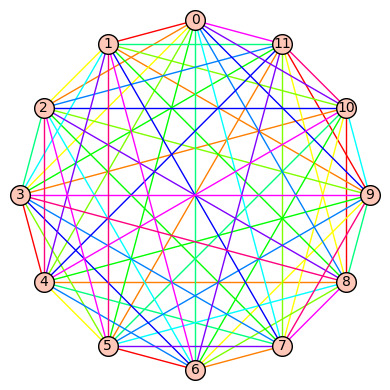
\includegraphics[scale=0.7, keepaspectratio=true]{k12-12colors.jpeg}
			\captionof{figure}{Uma coloração do $K_{12}$ com 12 cores.} 
			\label{fig:K12} 
	\end{center}
	
	\subsection{Uma família infinita de valores de $n$}
	Nesta subseção, calculamos o valor exato de $f_2(n, K_3)$ para uma família infinita de $n$ pares, que é o primeiro resultado mais abrangente conhecido para o problema.

  \begin{teorema}\label{teo:seq-f2}
        Dado $t$ um inteiro positivo, se $n=3^t + 1$, então $f_2(n,K_3) = n-1$.
   \end{teorema}
    \begin{proof}
        Vamos construir uma coloração própria de arestas de $K_n$ sob a condição de $n=3^t+1$ e mostrar que tal coloração não possui triângulos repetidos disjuntos em vértices.
        
        Destaquemos um vértice $u \in K_n$ de maneira que todos os  $3^t$ vértices restantes são elementos de  $\ZZ_3^t = \{x=(x_1, \dots, x_t) \colon x_i \in \ZZ_3, \ \forall i \in [t]\}$.
        
        Definimos a seguinte coloração $\chi \colon E(K_n) \rightarrow \{0,1,2\}^t = \ZZ_3^t$:
        \[
            \chi(\{x,y\}) = 
                \left\{\begin{matrix}
                (2x_1, \cdots, 2x_t) \mod 3, & \text{ se } y = u \\
                (x_1+y_1, \cdots, x_t+y_t) \mod 3, & \text{ se } u \notin \{x,y\},
                \end{matrix}\right.
        \]
        onde operamos a congruência % $\mod 3$
        a cada componente da $t$-tupla.
        
        A coloração $\chi$ obviamente utiliza até $n = 3^t$ cores pela construção sobre $\ZZ_3^t$. 
        Notemos também que $\chi$ é uma coloração própria.
        De fato, se duas arestas adjacentes e diferentes $e= \{x,y\}$ e $f=\{x,z\}$ recebem a mesma cor por $\chi$, então
        \begin{itemize}
            \item \textbf{Caso 1:} se $x = u$, então teríamos $2y_i = 2z_i$ para cada $i \in [t]$, logo, $y = z$, uma contradição;
            \item \textbf{Caso 2:} se $x \neq u$, então teríamos que $x_i + y_i = x_i + z_i$ (quando $y$ e $z$ são ambos diferentes de $u$) para cada $i \in [t]$, ou teríamos que $2x_i = x_i+z_i$ (se, s.p.g., $y = u$) para cada $i \in [t]$.
            No primeiro caso, obteríamos $y =z$, no segundo por sua vez que $x = z$, e com isso, obtemos outra contradição.
        \end{itemize}
        Resta-nos provar que $\chi$ não gera triângulos disjuntos repetidos em cores.
        Vamos supor, por contradição, que existem dois triângulos disjuntos com o mesmo conjunto de cores.
        
        Primeiro, suponha que ambos os triângulos não contém o vértice $u$ e os chamemos de $\{x,y,z\}$ e $\{a,b,c\}$, respectivamente, de cores $\alpha, \beta, \gamma$. Pela definição de $\chi$ podemos escrever para cada $i \in [t]$ que
        \[
            \left\{\begin{matrix}
            \alpha_i = a_i +b_i\\ 
            \beta_i = b_i+c_i\\ 
            \gamma_i = c_i+a_i
            \end{matrix}\right.
            \implies a_i = -\alpha_i+\beta_i-\gamma_i.
        \]
        De maneira análoga, $b_i$ e $c_i$ são determinados. 
        Resolvendo o mesmo sistema de equações para $x_i, y_i$ e $z_i$,
        concluímos que $a_i = x_i$ para cada $i \in [t]$.
        Isto implica que $a = x$ e contradiz que os triângulos são disjuntos.
        
        Agora, suponha que algum dos triângulos repetidos contém $u$, a saber, são $\{x,y,u\}$ e $\{a,b,c\}$ de cores $\alpha, \beta, \gamma$. 
        Disso temos para cada $i \in [t]$ que
        \[
            \left\{\begin{matrix}
            \alpha_i = x_i+y_i = a_i +b_i\\ 
            \beta_i = 2y_i = b_i+c_i\\ 
            \gamma_i = 2x_i = c_i+a_i
            \end{matrix}\right.
            \implies 
            \left\{\begin{matrix}
            2a_i = \alpha_i - \beta_i + \gamma_i\\ 
            2y_i = \alpha_i - \beta_i + \gamma_i
            \end{matrix}\right.
        \]
        que em $\ZZ_3$ implica em $y_i = a_i$, para cada componente $i$. Logo, $a = y$ contradizendo que os vértices da repetição  são disjuntos.
    \end{proof}
    
    \subsection{Problemas em aberto}
\label{subsec:repeated-prob}

        O parâmetro $f_2(n, K_3)$ com $n$ par continua a ser não compreendido sobre a existência de mais algum padrão em $\{n-1,n,n+1\}$ com outras sequências numéricas (Tabela \ref{tab:valores}).
        Variar o número de cópias de outros e também os grafos fixados forma um campo aberto a ser explorado.
        Janzer \cite{janzer2020rainbow} provou um resultado mais geral sobre repetições de ciclos pares, que em particular diz  $f_2(n, C_4) = \Omega(n)$, enquanto Conlon e Tyomkin \cite{conlontyomkyn} verificaram que $f_2(n, C_4) = O(n^{3/2})$. Resta-nos a seguinte pergunta:
        
        \begin{questao}\label{q:repeated-C4}
            Dado $n$ natural, $f_2(n, C_4) = \Theta(n)$?
        \end{questao}

  \begin{table}[] 
        \begin{tabular}{|l|lllllllllll}
        \hline
        $n$ & 4 & 6 & 8 & \text{\color{blue}10} & 12 & 14 & $\cdots$ & 26 & \text{\color{blue}28} & 30 & $\cdots$ \\ \hline
        $f_2(n, K_3)$ & 3 & 7 & 9 & \text{\color{blue}9}  & 12 & \text{\color{red}?}  & $\cdots$ & \text{\color{red}?}  & \text{\color{blue}27} & \text{\color{red}?}  & $\cdots$ \\ \hline
        \end{tabular}
        \caption{Valores de $f_2(n,K_3)$, em azul seguem do Teorema \ref{teo:seq-f2}.}\label{tab:valores}
\end{table}
 
 Conlon e Tyomkin \cite{conlontyomkyn} provaram que para árvores $T$ com $m$ arestas, existe alguma constante $k_0 = k_0(T)$ tal que para todo $k \geq k_0$ vale $f_k(n,T) = \Theta(n^{\frac{m+1}{m}})$. Os autores deixam a seguinte questão:
 
 \begin{questao}\label{q:repeated-T}\cite{conlontyomkyn}
     Qual o menor valor de $k_0$ tal que para todo inteiro $k \geq k_0$, vale $f_k(n,T) = \Theta(n^{\frac{m+1}{m}})$? 
 \end{questao}
 
 Um grafo $r$-partido completo é um grafo $r$-partido em que existe uma aresta para cada par de vértices de diferentes conjuntos independentes;
 se existem $n_1, \ldots, n_r$ vértices nos $r$ conjuntos independentes, denotamos o grafo $r$-partido completo por $K_{n_1, \ldots, n_r}$.
 Uma primeira generalização do problema de computar o parâmetro $f_k(n,H)$ é mudar o grafo base de coloração de $K_n$ para $K_{{\underbrace{n, \ldots, n}_{\text{$r$ vezes}}}}$, escrevemos o novo parâmetro por $f_k^r(n,H)$.

É direto que $f_k(n,H) = f_k^1(n,H)$ e que $f_k^2(n, K_3)= n$, pois grafos bipartidos não contêm triângulos e a coloração própria de $E(K_{n,n})$ utiliza $n$ cores. A questão levantada por nós é a seguinte:

\begin{questao}\label{q:tripartido}
    Dado $n$ natural, qual o valor de $f_2^3(n, K_3)$?
\end{questao}
 

\section{Um problema do tipo anti-Ramsey}\label{sec:anti}

Dada uma coloração das arestas de um grafo $G$, dizemos que uma cópia de um grafo $H$ em $G$ é \emph{rainbow} se não existem duas arestas de $H$ com a mesma cor.
%
Dados grafos~$G$ e~$H$, estamos interessados na seguinte propriedade denotada por ${G\rbarrow H}$: para toda coloração \textit{própria} das arestas de~$G$ (com uma quantidade arbitrária de cores),
existe uma cópia rainbow de~$H$ em~$G$, i.e., um subgrafo de $G$ isomorfo a $H$ com todas as arestas de cores distintas.

Ressaltamos uma definição importante que é objeto de investigação no grafo aleatório nesta seção.
Uma função $\hat{p}: \mathbb{N} \rightarrow [0,1]$ é chamada de \textit{função limiar} para uma propriedade
$\cP$ no $G(n,p)$ se 
\[
  \lim_{n\to\infty}\mathbb{P}\left(G(n,p) \in \cP\right)
  =
  \begin{cases}0&\text{if }p \ll \hat p, \\
    1&\text{if }p \gg \hat p.
  \end{cases}
\]
Os limites na definição acima de função limiar são chamados de $0$-\emph{statement} e $1$-\emph{statement}, respectivamente. 
Uma vez que os limiares são determinados por ordem de magnitude, vamos nos referir aos limiares $\hat{p}$ como \emph{o limiar} da propriedade $\cP$.
A propriedade anti-Ramsey ${G\rbarrow H}$ é monótona em grafos aleatórios, logo, admite uma função limiar, que nós denotamos por $\hat{p}_H$. 


No que segue precisamos considerar as densidades de um grafo: a \emph{$2$-densidade máxima} de um grafo $H$, denotada por~$m_2(H)$, é definida como 
\begin{equation*}
  m_2(H)=\max\left\{\frac{|E(J)|-1}{|V(J)|-2}\colon J\subset H,\;|V(J)|\geq3\right\},
\end{equation*}
onde assumimos~$|V(H)|\geq3$, e 
\[
    m(H) = \max\left\{\frac{|E(J)|}{|V(J)|}\colon J\subset H,\;|V(J)|\geq1\right\},
\]
é a \emph{densidade máxima} de $H$, a qual frequentemente vamos chamar só de densidade de $H$.



\subsection{Resultados existentes}

Em~\cite{KoKoMo12}, o orientador e colaboradores provaram o seguinte resultado: a propriedade anti-Ramsey $G(n,p)\rbarrow H$ vale assintoticamente quase certamente sempre que $p\gg n^{-1/m_2(H)}$ para todo grafo fixo~$H$. Em outras palavras, garante-se em termos da $2$-densidade máxima de um grafo $H$ um limitante superior para a função limiar $\hat{p}_H$, como enunciado a seguir.

\begin{teorema}[Kohayakawa, Konstadinidis e Mota~\cite{KoKoMo12}]
    \label{teo:conditional}
         Seja $H$ um grafo fixo. Então existe uma constante $C>0$ tal que, para $p=p(n)\geq Cn^{-1/m_2(H)}$, assintoticamente quase certamente temos ${G(n,p)\rbarrow H}$. 
         Em particular, $\hat{p}_H \leq n^{-1/m_2(H)}$.
  \end{teorema}
    
Dado o Teorema \ref{teo:conditional} e sabendo que a $2$-densidade máxima tem um papel fundamental em Teoria de Ramsey, é natural perguntar se $n^{-1/m_2(H)}$ é função limiar para a propriedade $G(n,p)\rbarrow H$ para qualquer grafo $H$.
No entanto, em \cite{KoKoMo16+}, foi obtida uma resposta negativa para essa pergunta, onde os autores exibiram uma família infinita de grafos cuja função limiar é inferior a $n^{-1/m_2(H)}$.
Porém a 2-densidade máxima se relaciona, de fato, à função limiar para alguns grafos $H$, como foi provado por Nenadov,
Person, Škorić e Steger~\cite{NePeSkSt14}.

\begin{teorema}[Nenadov, Person, Škorić e Steger~\cite{NePeSkSt14}]
\label{teo:nen}
  Seja $H$ um ciclo de pelo menos $7$ vértices um grafo completo de pelo menos $19$ vértices. 
  Existe uma constante $c > 0$ tal que se
  $p\leq cn^{-1/m_2(H)}$, 
  então com alta probabilidade $G(n,p)\not\rbarrow  H$.
\end{teorema}

%% Comentamos a seguir o trabalho que fecha o limiar da classe de ciclos a partir de $C_4$, e em seguida o trabalho que trata de grafos completos a partir de $K_4$.

O Teorema \ref{teo:nen} foi estendido para ciclos (\cite{barros2021anti}) e grafos completos (\cite{kohayakawa2019anti}) com mais de 5 vértices.

\begin{teorema}    
[\cite{barros2021anti},
\cite{kohayakawa2019anti}]
\label{teo:cyclecomplete} 
Se $H$ é um ciclo ou um grafo completo de pelo menos $5$ vértices, 
então $\hat{p}_{H} \geq n^{-1/m_2(H)}$. 
Além disso, $\hat{p}_{C_4} = n^{-3/4}$ 
e $\hat{p}_{K_4} = n^{-7/15}$.
\end{teorema}
    
\begin{lema}\label{lema:rbciclos}\cite{barros2021anti}
         Sejam $\ell \geq 5$ um inteiro e $G$ um grafo tais que
         $m(G) < (\ell-1)/(\ell-2)$. 
         Então, $G \not\xrightarrow[]{rb} C_\ell$.
\end{lema}
    
A essência da prova do Lema \ref{lema:rbciclos} está em usar uma estratégia de coloração própria nas arestas dos ciclos $C_\ell$ contidos no grafo $G$, de modo que qualquer ciclo $C_\ell$ tenha duas arestas coloridas com a mesma cor.
%
Para isso, os autores definem o que chamam de componente de ciclos dentro de $G$ como uma sequência crescente de subgrafos $(H_1, \ldots, H_t)$ em $G$, em que a cada subgrafo existe um $C_\ell$ em $H_{i+1}$ que não está em $H_i$, para $1 \leq i < t$, com alguma interseção não-nula com $H_i$.
%
Observam que tal sequência impõe certas configurações restritas de como os novos ciclos aparecem entre os subgrafos, assim trabalhando na combinação dessas configurações detalham alguns casos de como colorir arestas dessa sequência de subgrafos para evitar $C_\ell$ rainbow.
     Parte das ideias desse artigo são retomadas nas demonstrações descritas na próxima subseção.
 
 
   Para provar que o limiar para que $G(n,p) \rbarrow K_\ell$, com $\ell \geq 5$ é igual a $p = n^{-1/m_2(K_\ell)} = n^{- 2/(\ell+1)}$, os autores provam o seguinte lema.
   % destacamos que o grafo $K_4$ tem um limiar diferente e é tratado à parte no mesmo artigo.
   
   \begin{lema}\label{lema:rbcomplete}\cite{kohayakawa2019anti}
         Sejam $\ell \geq 5$ um inteiro e $G$ um grafo tais que 
         $m(G) < (\ell+1)/2$.
         Então, $G \not\xrightarrow[]{rb} K_\ell$.
    \end{lema}
    Para demonstrar o Lema \ref{lema:rbcomplete}, é suficiente mostrar que todo grafo $G$ com $m(G) < (\ell+1)/2$  admite colorações próprias que evitam $K_\ell$ rainbow. 
    A primeira observação é que é suficiente considerar $G$ como um grafo onde toda aresta está contida em algum $K_\ell$, pois são elas que importam em uma coloração sem $K_\ell$ rainbow. 
    Os autores notam que a densidade limitada de $G$ implica na existência de ao menos um vértice $v$ de grau $\ell$, e, com esse vértice destacado apresentam uma prova indutiva na quantidade de vértices de $G$: consideram na hipótese indutiva ao subgrafo $G_v$ de $G$ obtido após remover $v$ e seus vizinhos que participam de algum $K_\ell$ em comum.
    
    Antes de dar a propriedade a ser preservada na indução, com argumentos usando a densidade limitada nos subgrafos de $G$, são analisadas as possíveis configurações da vizinhança de $v$ quanto a formar cliques que se interceptam. 
    %% O parâmetro auxiliar $b(G)$ que contabiliza a proporção de arestas coloridas é relacionado a essas configurações e, com ele, a indução de $G_v$ para $G$ é construída notando que para diferentes valores em $b(G)$, cada $K_\ell$ do grafo será não-rainbow.
 
 
\subsection{Limiar para grafos bipartidos completos}

    Nesta subseção queremos provar para grafos bipartidos completos um resultado semelhante ao que foi comentado anteriormente sobre ciclos e grafos completos, a saber, a propriedade anti-Ramsey de grafos bipartidos em grafos aleatórios.
    Ou seja, dados os inteiros $\ell,r \geq 3$, pretendemos verificar que o limiar para a propriedade $G(n,p) \xrightarrow[]{rb} \K$ é dado por $n^{-1/m_2(\K)}$.

    Note que como toda coloração própria de arestas de uma estrela $K_{1,r}$ é obrigatoriamente rainbow, então
    o limiar da propriedade anti-Ramsey no caso de estrelas $K_{1,r}$ coincide com o limiar para que uma estrela $K_{1,r}$ apareça em grafos aleatórios.

    O caso de grafos bipartidos completos $K_{2,r}$, para $r\geq 1$ (o caso $r=2$, que corresponde ao $C_4$, é coberto pelo
    Teorema~\ref{teo:cyclecomplete}),
    nós provamos que $K_{2,3r-2} \rb K_{2,r}$, 
    o que implica que  a presença de um $K_{2,3r-2}$ no
    $G(n,p)$ guarante a existência de uma cópia rainbow de $K_{2,r}$ em qualquer coloração própria de arestas de~$G(n,p)$.  

     \begin{teorema}\label{teo:below} Seja $r\geq 1$ um inteiro, então
    $K_{2,3r-2} \rb K_{2,r}$.
     \end{teorema}
     \begin{proof} Nós provamos este resultado por indução em $r$. 
     O resultado claramente vale para $r=1$ pela coloração própria de $K_{2,1}$ ser rainbow. 
     Fixe $r\geq 2$ e suponha que $K_{2,3r-5} \rb K_{2,r-1}$. 
     Seja $G:=K_{2,3r-2}$ com partes $X$ e $Y$, onde $|X|=2$ e $|Y|=3r-2$, e considere uma coloração própria de suas arestas.
     Então, como ela contém uma cópia de $K_{2,3r-5}$ e $K_{2,3r-5} \rb K_{2,r-1}$, então existe uma 
     cópia rainbow de $H_A:=K_{2,r-1}$ em $G$.
     Agora, considere  o subgrafo $H_B:=K_{2,2r-1}$ de $G$, disjunto de $H_A$, com partes $X$ e $B$. 
     Uma vez que $H_A$ é colorido com $2r-2$ cores e $B$ possui
    $2r-1$ vértices, existe ao menos um vértice $b\in B$ tal que
    duas arestas de $H_B$ incidem em $b$ e não são usadas em $H_A$. 
    Portanto, a cópia de $K_{2,r}$ obtida por adicionar $b$ em $H_A$ é rainbow.
     \end{proof}
    
    Agora, como  o limiar para
    $K_{2,3r-2}\subset G(n,p)$ é $n^{-1/m(K_{2,3r-2})}$ e
    $m(K_{2,3r-2}) = (6r-4)/3r < (\ell r - 1)/(\ell+r-2) =
    m_2(K_{\ell,r})$, 
    temos que $K_{2,3r-2}$ força um limite superior menor do que
     $n^{-1/m_2(K_{2,r})}$, i.e., nós concluímos que
    \[ 
      \hat{p}_{K_{2,r}} \ll n^{-1/m_2(K_{2,r})}.
    \]

    Nosso principal resultado (Teorema \ref{teo:mainrb}) mostra que, diferentemente do limiar de $K_{2,r}$,
    o limiar $\hat{p}_{\K}$ quando $\ell,r \geq 3$ é de fato da ordem 
    $n^{-1/m_2(\K)} = n^{-(\ell+r-2)/(\ell r-1)}$.
    A partir do Teorema \ref{teo:conditional}, temos o limite superior $\hat{p}_H \leq n^{-1/m_2(H)}$ para todo grafo $H$, e com isso, para determinarmos o limiar de $\hat{p}_{\K}$ é suficiente mostrar que 
    $\hat{p}_{\K}\geq n^{-(\ell+r-2)/(\ell r - 1)}$.

    \begin{teorema}\label{teo:mainrb} 
    Sejam $\ell,r \geq 3$ inteiros. 
    Então $\hat{p}_{K_{\ell,r}}\geq n^{-(\ell+r-2)/(\ell r - 1)}$.
    \end{teorema}

    %%yyyyy
    Uma vez que $\K$ um grafo estritamente 2-balanceado, a partir do Teorema XX, podemos deduzir o Teorema \ref{teo:mainrb} a partir do seguinte resultado que é provado na Subseção ZZ.
    
    \begin{teorema}\label{lemma:main} 
        Sejam $\ell,r \geq 3$ inteiros e
        $G$ um grafo. 
        Se $m(G) < m_2(\K)$, então $G \not\rb \K$.
    \end{teorema}

    %%%yyyyy
    Na Subseção \ref{sec:rbestrut} provamos alguns resultados estruturais que caracterizam como as cópias de $\K$ aparecem no grafo com densidade máxima limitada superiormente por $m_2(\K)$.
    Na Subseção YY provamos o Teorema \ref{lemma:main}.

\subsection{Resultados Estruturais}
\label{sec:rbestrut}

     A fim de provarmos o Teorema~\ref{lemma:main}, dado um grafo $G$ tal que
     $m(G) < m_2(\K)$, 
     precisamos obter coloração de arestas de $G$ sem cópias rainbow de~$\K$. 
     Para isto, precisamos pensar nas interseções de arestas das cópias de grafos bipartidos completos, dado que colorir tais arestas de maneira a evitar $\K$ rainbow pode exigir uma coloração engenhosa. 
     
     Começamos com a seguinte proposição cuja demonstração é obtida
     pela aplicação do \textit{argumento de densidade}, este último  será muito utilizado nas provas desta seção.
    %xxxxx Como estamos interessados em grafos $G$ tais que  $m(G) < m_2(\K) = (\ell r - 1)/(\ell+r-2)$,  we state a simple observation that will be helpful when analyzing subgraphs of $G$.  
    Dado um grafo $G$, denotamos uma cópia de um grafo bipartido completo em $G$ com partes $A$ e $B$ por $G[A,B]$.
    
    \begin{proposicao}
        \label{lemma:inter_a} 
    Sejam $r\geq \ell\geq 3$ inteiros, $G$ um grafo, $G[A_1,B_1]$ e $G[A_2,B_2]$ cópias de $K_{\ell,r}$ em $G$. 
    Se $m(G) < m_2(\K)$ e
    $A_i \cap B_j = \emptyset$ 
    para $1\leq i,j\leq 2$, então o grafo bipartido completo
    $G[A_1\cap A_2, B_1\cap B_2]$ é uma cópia de $K_{a,b}$ tal que
      \begin{equation}
         \label{eq:pairs-ab} 
    	 \frac{2\ell r - ab}{2\ell + 2r - (a+b)} <
    \frac{\ell r - 1}{\ell + r - 2}.
      \end{equation}
      \end{proposicao}
    \begin{proof}
    Sejam $H_1:=G[A_1,B_1]$ e $H_2:=G[A_2,B_2]$.
    Da mesma forma, seja $H:= G[a,b]$, onde $a = A_1\cap
    A_2$ e $b = B_1\cap B_2$.  
    Uma vez que 
    $v(H_1 \cup H_2) = (\ell + r) +
    (\ell-a) + (r - b) = 2\ell + 2r - (a+b)$ 
    e $e(H_1 \cup H_2) = \ell r + (\ell-a)r + a(r-b)$, 
    da densidade $m(H) \leq m(G)$ e de $H\subset H_1\cup
    H_2$, temos que
      \begin{equation*} 
      \frac{\ell r + (\ell-a)r + a(r-b)}{2\ell + 2r -
    (a+b)} = \frac{2\ell r - ab}{2\ell + 2r - (a+b)} < \frac{\ell r -
    1}{\ell + r - 2},
      \end{equation*}
      o que conclui a prova.
    \end{proof}
    
    Faremos frequente aplicação, direta ou indiretamente, da Proposição~\ref{lemma:inter_a} em nossas provas.
     
     Vamos seguir uma estratégia próxima à encontrada em \cite{barros2021anti}, da propriedade anti-Ramsey de ciclos, que analisou interseções de arestas entre ciclos no grafo a ser colorido de densidade limitada.
     Dado um grafo $G$, sejam $H_1, \ldots, H_t$ uma sequência crescente de subgrafos de $G$ tal que
    $H_1$ é uma cópia de $\K$ e, para cada $1 < i \leq t$, temos $H_{i-1} \subseteq H_i$ e existe alguma cópia de $\K$ em $H_{i}$ com interseção de arestas não-nula com $H_{i-1}$. 
    Ou seja, existe um $K \cong \K$ em $H_{i}$ tal que $K \not\subset H_{i-1}$ e $E(K) \cap E(H_{i-1}) \neq\varnothing$.
     Observe que a inclusão de uma cópia de $\K$ em $H_{i-1}$ pode até formar outras cópias de $\K$ em $H_{i}$ não presentes em $H_{i-1}$, sendo este um detalhe importante quando nos voltarmos para a coloração de $G$.
     
     Se a sequência $H$ for maximal, isto é, não pode mais ser estendida em $G$, ela será chamada de $\K$-componente.
     Queremos realizar uma coloração própria parcial da sequência $(H_1, \ldots, H_t)$ em que é possível evitar $\K$ rainbow.
 
 Na Proposição \ref{lemma:inter_a}, dado um grafo $G$ com
 $m(G) < m_2(\K)$, nós descrevemos os tamanhos dos subgrafos obtidos nas cópias $G[A_1,B_1]$ e $G[A_2,B_2]$ de $K_{\ell,r}$ em $G$ sob a condição $(A_1\cup A_2)\cap(B_1\cup B_2) = \emptyset$.
 A próxima proposição lida com o caso em que $A_1\cup A_2$ intersecta a $B_1\cup B_2$, sua prova segue a mesma ideia da Proposition \ref{lemma:inter_a} com um argumento de densidade similar à desigualdade \ref{eq:pairs-ab}, porém apresenta uma solução única para esta, o que força uma configuração específica de intersecções de arestas.


    \begin{proposicao}\label{aff:casoP1}
       Sejam $3\leq \ell \leq r$ inteiros, 
      $G$ um grafo, e $K_1 \cong G[A, B]$ uma cópia de $\K$ em $G$.
      Se $m(G) < m_2(\K)$ e existe em $G$ uma outra cópia
        $K_2 \cong \K $ que intercecta arestas de $K_1$ tal que 
        $(E_G[A] \cup E_G[B]) \cap K_2 \neq \varnothing$, 
        então $K_2$ contém uma cópia de $K_{\ell-1,r-2}$ disjunta de $K_1$.
    \end{proposicao}
     \begin{proof}
         Seja $K$ uma cópia de $\K$ em $G$ com partes $A$ e $B$, queremos verificar se existe em $G$ o subgrafo $K'$ também cópia de $\K$ com partes $X$ e $Y$, onde pelo menos $A \cap X \neq \varnothing$ e $A \cap Y \neq \varnothing$.
         
         Sejam $X' = X\setminus A$,  $B' = B\cap Y$, $A' = A \cap Y$ e $Y' = Y \setminus (B\cup A')$, 
         onde
         $X'$ tem $x$ vértices, $A'$ tem $a$ vértices, $B'$ tem $b$ vértices e $Y'$ tem $y$ vértices.
         
         É evidente que $a \geq 1$, $b \geq 1$, e também que $a + b+y = \ell$ e $a + (\ell-x) \leq \ell$ são condições da construção. 
         Reunindo essas informações com a densidade a seguir 
         
         \[
            m(K \cup K') = \frac{\ell r + xr + (\ell-x)(a+y)}{\ell+r+x+y}
            < \frac{\ell r - 1}{r+\ell-2},
         \]
         obtemos que a única solução é $b=1$, $x = \ell-1$, $a=1$ e $y=r-2$. 
         De $X'$ e $Y'$ obtemos $K_{\ell-1, r-2}$ em $K'$ vértice disjunto de $K$.
         Uma parametrização semelhante usando arestas internas de ambos os conjuntos $A$ e $B$ não gera soluções.       
         %% \text{\color{red} verificar grafico e completude}
     \end{proof}
     
     Uma informação útil sobre a configuração dada na Proposição \ref{aff:casoP1} 
     % é de que ela limita a existência de uma interseção do tipo $K_{1,1}$ com outro $\K$. 
     % Logo, seria 
     é que tal configuração é densa o suficiente para ser uma $\K$-componente isolada do grafo $G$, pois não permite intersecções com mais grafos bipartidos completos.
     
     Nós reiteramos que uma intersecção entre duas cópias de $\K$ em $G$ é da forma $K_{a,b}$ para alguns inteiros $a$ e $b$. 
	 O grafo $G$ pode conter uma intersecção de múltiplas cópias de
    $\K$, dado que este caso seria um subgrafo de $K_{\ell+x,r+y}$ onde $x$ ou $y$ são inteiros positivos, e, como veremos, esta intersecção múltipla pode afetar a $\K$-componente de $G$. 
    
    Notamos que uma sequência de $\K$ que se interceptam em arestas possui menor densidade se as intersecções entre cada par de $\K$ da sequência forem da forma $K_{1,1}$. 
     Dada esta informação, computamos limite inferior para a densidade de uma sequência de $\K$ em $G$, e obtivemos restrições sobre a estrutura das intersecções de arestas na $\K$-componente de $G$, como é apresentado no seguinte fato.
     
      \begin{fato}\label{fato:ciclos}
        Sejam $3\leq \ell \leq r$ inteiros e seja $G$ um grafo tal que $m(G) < m_2(\K)$.  
        Dada uma $\K$-componente $(H_1, \ldots, H_t)$ de $G$, 
        então o grafo bipartido $K \cong K_{\ell+s, r+w}$ contido em $H_i$, mas não em $H_{i-1}$ é tal que 
        $E_G(K) \cap E_G(H_j) = \varnothing$
        para todo $1 \leq j < i-1$ e algum valor de $0\leq s < \ell$, $0\leq w < r$ .  
  \end{fato}
\begin{proof}
        As interseções entre grafos bipartidos completos de $G$ da forma $K_{1,1}$ são as que permitem mais arestas, pois apresentam menor densidade. 
        Suponha para um $s$-ciclo no grafo de interseção $\mathcal{I}(G)$ -- o que representa uma cadeia de $\K$'s em $G$ --  considerando só interseções da forma $K_{1,1}$.
        Teríamos em termos de densidade em $G$ dessa cadeia de interseções que
        \[
            \frac{s\ell^2 - s}{s2\ell - 2s} =  \frac{\ell^2 - 1}{2\ell - 2}
            \not\leq \frac{\ell+1}{2}. 
        \]
        Logo, o grafo de interseção não contém ciclos considerando o conjunto $I_\ell \setminus \{(\ell-2,\ell), (\ell-1,\ell)\}$.
       % \text{\color{red} argumentar que os vértices densos internos não mudam o fato, repetem a conta}.
       Tratar os múltiplos $\K$'s que podem ser gerados por intersecções do tipo $\{(\ell-2,\ell), (\ell-1,\ell)\}$ como um único vértice de $\mathcal{I}(G)$ torna tal grafo acíclico pelo mesmo argumento.
\end{proof}

      Nós usaremos as consequências da Proposição \ref{lemma:inter_a} e, com a análise de densidade de múltiplas intersecções entre grafos bipartidos $\K$ na sequência de subgrafos $(H_1, \ldots, H_t)$, obtemos um resultado que caracteriza a confuguração estrutural da cópia de $\K$ que aparece entre $H_{i-1}$ e $H_i$.
     Antes, definimos os parâmetros $e_j$ e $v_j$, para cada $1 \leq j \leq i$:
     \begin{itemize}
         \item $e_j$ é o número de arestas em $E(H_{j}) \setminus E(H_{j-1})$;
         \item $v_j$ é o número de vértices em $V(H_{j}) \setminus V(H_{j-1})$. 
     \end{itemize}
     
     Note que $v_j \leq \ell+r-2$, pois por intersecção de arestas, o $\K$ entre $H_{j-1}$ e $H_{j}$ contém ao menos uma aresta de $H_{j-1}$, o que exige dois vértices em $H_{j-1}$. 
     Os $v_{j}$ vértices formam $K_{\ell-a,r-b}$ em $H_{j}$, com $0 \leq a\leq \ell$ e $0\leq b\leq r$, onde $a,b$ são inteiros e ambos não assumem o valor máximo (mínimo) ao mesmo tempo, e $v_{j} = \ell+r-a-b$.
 

  Para um conjunto de vértices $X = \{x_1, \ldots, x_\ell\}$, dados inteiros $1 \leq a \leq b \leq \ell$, denotamos por $X_a^b$ o subconjunto $\{x_a, \ldots, x_b\}$ de $X$. 

    Dada uma $\K$-componente $(H_1, \ldots, H_t)$ de $G$, 
    seja $K = [X, Y]$ uma cópia de $\K$ em $H_i$, mas não em $H_{i-1}$, 
    onde $X = \{x_1, \ldots, x_\ell\}$ e $Y=\{y_1, \ldots, y_r\}$, para algum $2\leq i\leq t$
    e considere os inteiros $1 \leq j, s \leq \ell$ e $1 \leq k,w \leq r$.  
    Sejam $0 \leq p \leq \ell-j$, $0\leq q \leq r -k$ e $z = s+w$ inteiros, 
     definimos as seguintes \emph{configurações} de $K$: 
       \begin{enumerate}
       \item[$(A_{jk})_{pq}$]\label{configA} 
        os conjuntos de vértices $X$ e $Y$ são tais que $K$
    contém o subgrafo
    $K_{j,k} = \big[X_1^j, Y_1^k\big]$ in $H_{i-1}$, 
    ele também forma um 
    $K_{p,q} = \big[X_{j+1}^{j+p}, Y_{k+1}^{k+q}\big]$
    com  vértices de $H_{i-1}$, onde $X$ e $Y$ são completados com vértices de
    $X_{j+p+1}^\ell$ e $Y_{k+q+1}^r$ em $H_i$, respectivamente;
                
       \item[$(B_{sw})$]\label{configB} 
        Existem conjuntos de vértices $X,Y$ em $H_{i-1}$ e $Z_1, Z_2$ em $H_i$, tais que
      $K_{s,w} = [Z_1, Z_2]$ e 
      $K_{\ell+s,r+w}= [X\cup Z_1, Y\cup Z_2]$ que contém~$K$.
      \footnote[1]{Um caso especial se dá quando $z = 0$ e 
     ou $Z_1$ ou $Z_2$ é um conjunto unitário, com isso, $V(H_i) = V(H_{i-1})$.}
       \end{enumerate}

    Nós também dizemos que $H_i$ é de uma das configurações, $(A_{jk})_{pq}$ ou $(B_{sw})$, 
    quando $H_i = H_{i-1} \cup K$ e satisfaz as condições acima. 
	De maneira geral, dizemos que $K$ é do \textit{tipo A} se $K$ é da configuração $(A_{jk})_{pq}$, analogamente,
		$K$ é do \textit{tipo B} se $K$ é de uma configuração $(B_{sw})$.
  
  \begin{figure}[htb] \centering 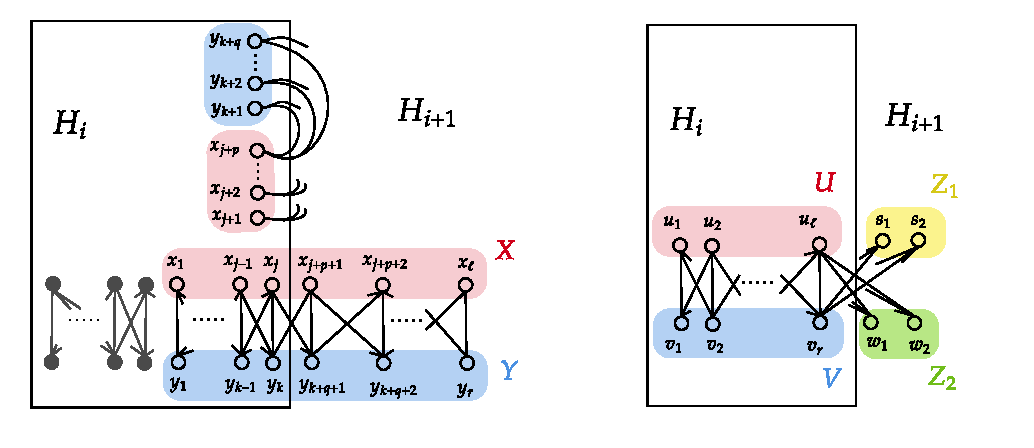
\includegraphics[]{configAB_KLL.pdf}
   \caption{Configurações $(A_{jk})_{pq}$ e $(B_{sw})$ de um $\K$ contido em $H_i$, mas não em $H_{i-1}$.}
   \label{fig:configKLL}
 \end{figure}
 
  
 \begin{lema}\label{lema:config}
        Sejam $3\leq \ell \leq r$ inteiros, e $G$ um grafo tal que $m(G) < m_2(\K)$, 
     e $H = (H_1, \ldots, H_t)$ uma $\K$-componente de $G$.  
    Então,  vale para cada $2\leq i \leq t$: 
    se $K = [X, Y]$ é uma cópia de $\K$ em
    $H_i$ e não em $H_{i-1}$, 
    então $K$ é do tipo A ou B.   
    \end{lema}
\begin{proof}
        Vamos provar o resultado para todos valores possíveis de $v_i$, i.e., $0\leq v_i \leq \ell+r-2$ e para o número de novos $\K$ adicionados a $H_i$.
       
    Primeiro, construímos conjuntos auxiliares que descrevem as intersecções de arestas de grafos bipartidos em $G$.   
    Dados os inteiros positivos $\ell$ e $r$, denote por
    $\mathcal{S}_{\ell,r}$ o conjunto de pares $\{a,b\}$ tal que a Proposition~\ref{eq:pairs-ab} vale.  
    Definimos os conjuntos $\mathcal{S} = \left\{\{1,1\},\{1,2\},\{1,3\},\{2,2\}\right\}$ e
    \begin{equation*} 
    	\mathcal{S}_\ell =
    \left\{\mathcal{S},\{\ell-1,\ell-1\},\{\ell-2,\ell\},\{\ell-1,\ell\}\right\}.
    \end{equation*} 
    
    É fácil verificar da Proposição~\ref{lemma:inter_a} que os valores possíveis para $\mathcal{S}_{\ell,r}$ são apresentados a seguir.
     Para tanto, definimos os conjuntos de inteiros consecutivos 
     $\beta_1:=\{\lceil (\ell^2r - 4\ell r +
    \ell+2r)/((\ell-1)^2)\rceil,\dots, r-1\}$ 
    e
    $\beta_2:=\{\lceil
    (-\ell^2r +5\ell r - \ell-2r-1)/(r-\ell^2+3\ell-3)\rceil,\ldots, r\}$.
    
      \begin{itemize}
      \item [(i)] se $r=\ell = 3$ ou $r=\ell \geq 7$, então
    $\mathcal{S}_{\ell,r} = \mathcal{S}_\ell$;
      \item [(ii)] se $r=\ell = 4$, então $\mathcal{S}_{\ell,r} =
    \mathcal{S}_\ell \cup\big\{\{2,3\}\big\}$;
      \item [(iii)] se $r=\ell = 5$, então $\mathcal{S}_{\ell,r} =
    \mathcal{S}_\ell \cup\big\{\{2,3\},\{3,3\},\{3,4\}\big\}$;
      \item [(iv)] se $r=\ell = 6$, então $\mathcal{S}_{\ell,r} =
    \mathcal{S}_\ell \cup\big\{\{2,3\},\{3,3\},\{4,5\}\big\}$;
      \item[(v)] if $7 \leq \ell < r \text{ e } r > \ell^2-3\ell+3$,
    então $\mathcal{S}_{\ell,r} = \mathcal{S} \cup \{\{a,b\}: a=\ell\text{
    and }b\in \beta_1\}$;
       \item[(vi)] se $7 \leq \ell < r \text{ e } r \leq
    \ell^2-3\ell+3$, então $\mathcal{S}_{\ell,r} = \mathcal{S} \cup
    \{\{a,b\}: a=\ell\text{ e }b\in \beta_1;\text{ ou }a=\ell-1\text{
    e }b\in \beta_2\}$.
      \end{itemize}

    
    \medskip \textbf{Case 1.}
	Se $3 \leq v_i \leq \ell+r-2$ e somente uma cópia de $\K$ é adicionada para formar $H_i$.
   
    Seja $v_i= \ell+r-a-b$, onde $a,b$ são inteiros positivos.  
    Os $v_i$ vértices de $K \cong \K= [X,Y]$ formam o bipartido $K_{\ell-a,r-b}$ em $H_i$; a $\K$-componente é
    composta pelas intersecções de arestas de $K$ com $H_{i-1}$ formando $K_{j,k}$,
    onde $\{j,k\} \in \mathcal{S}$ (Proposição \ref{lemma:inter_a}).  
   
   Completamos a partição $[X,Y]$ tomando outros $p,q$ vértices em $H_{i-1}$ tais que um $K_{p,q}$ é gerado satisfazendo às condições de  $j+p = a$ e $k+q = b$. 
   
   Suponha que já haviam arestas em $K_{p,q}$  para algum $H_j$ na sequência de subgrafos com $j < i-1$.
   Logo, o novo $K$ adicionado teria interseção de arestas com algum outro bipartido completo $K'$, além do bipartido $K''$ que contém $K_{jk}$ em $H_{i-1}$.
   Assim, considerando o subgrafo $H_{i}$, teríamos que existe um caminho entre $K'$ e $K''$, e então $K$ 
   tem interseção com algum $H_j$ com $j<i-1$, o que contradiz o Fato \ref{fato:ciclos}.
  
     Então, as arestas de $K_{p,q}$ são adicionadas por $H_i$ na $\K$-componente e, nós obtemos a configuração~\hyperref[configA]{$(A_{jk})_{pq}$}. 
    Esta configuração forma um único $\K$ com $H_i$,  agora consideramos casos mais de um $\K$ aparece em $H_i$.

    Sejam $b_1, b_2$ inteiros positivos tais que $b_1 \in \beta_1$ ou $b_2 \in \beta_2$.
    
     \medskip \textbf{Case 2.} 
    Se $v_i \in [1, \max\{r - b_1, r+1-b_2\}]$ e existem múltiplas cópias de $\K$ entre $H_{i-1}$ e $H_i$.
	
   Seja $Z$ o conjunto com estes $v_i$ vértices, 
   se existe exatamente uma aresta em $Z$, digamos $uv$, então temos que
    $Z_1 = \{u\}$ e $v \in Z_2$ e, com isso,
    ~\hyperref[configB]{$(B_{1,w})$} é possível, onde $w = r-b_2$.
        
        Outro subcaso ocorre se não há arestas em $Z$, assim $Z_1 =
    \varnothing$ e obtemos a configuração~\hyperref[configB]{$(B_{0,w})$}, 
    onde $z = w = r-b_1$.
    
    Um caso excepcional ocorre quando $\ell = r$ e permite a
configuração~\hyperref[configB]{$(B_{2,0})$}.
   
 \medskip \textbf{Case 3.} 
	  Se $v_i = 0$ e existem múltiplas cópias de $\K$ entre $H_{i-1}$ e $H_i$. 
	  
	 Tem-se que toda nova aresta de $H_i$ se liga a vértices pré-existentes de $H_{i-1}$. 
      Se considerarmos somente a adição de arestas em um único $\K$ de $H_{i-1}$, veremos que não é possível criar outro bipartido $K$, pois pelo argumento de densidade temos que
    \[ 
		\frac{\ell r + e_i}{\ell+r} < \frac{\ell r-1}{r+\ell-2}.
    \]
	Isto implica sob as condições de $3 \leq \ell < r$ que 
	$e_i \leq (2\ell r -\ell-r)/(\ell+r-2) < \ell+r-2$, 
	tal quantidade $e_i$ é insuficiente para inverter dois vértices da partição no subgraph que resulte em outro $\K$.
    Com isso, vamos analisar intersecções em $H_{i-1}$ com mais de $\K$.
    
    Para as intersecções possíveis entre dois bipartidos completos $K'$ e $K''$, descritas na Proposição \ref{lemma:inter_a}, realizamos a  análise da seguinte desigualdade de densidades:

    \[
		\frac{2\ell r - e(K'\cap K'') + e_i}{2\ell+2r - v(K' \cap K'')} < \frac{\ell r- 1}{\ell+r-2}.
    \]
    
     Em particular, vemos que $K_{1,3}$, $K_{2,2}$ são intersecções justas, isto é, são subgrafos de $H_{i-1}$ cujo argumento de densidade requer $e_i=0$, i.e., não permitem acréscimo de arestas;
    e para $K_{\ell-2,r}$ temos $e_i < \ell$ que também não forma outro $\K$.
    %
     Já se a intersecção for $K_{1,1}$, para todos os valores de $\ell$ e $r$ temos que $e_i = \ell-1$, disso para gerar um novo $\K$ de $H_{i}$, basta escolher um vértice de fora da interseção e adicionar a ele $e_i$ arestas para formar $K_{\ell+1,r}$, logo, de configuração~\hyperref[configB]{$(B_{1,0})$}; analogamente, temos para $\ell \in
        \{r-1, r\}$ com $e_i = r-1$ a configuração
        ~\hyperref[configB]{$(B_{0,1})$}.
    %
    A interseção $K_{\ell-1, r-1}$ temos uma única solução $e_i=1$, e podemos dela obter $K_{\ell+1, r}$ ou $K_{\ell,r+1}$, logo, de configurações ~\hyperref[configB]{$(B_{1,0})$}
    e ~\hyperref[configB]{$(B_{0,1})$}, respectivamente.. 
    %
     A intersecção $K_{1,2}$ admite $e_i = \ell-1$, se $r > \ell^2 - 3\ell+3$ e isso permite a configuração~\hyperref[configB]{$(B_{1,0})$}.
    %
    As outras intersecções mais gerais, a saber $K_{\ell-1, r-b}$, $K_{\ell,b_1}$ e $K_{\ell-1, b_2}$, precisam dos limites de $e_i < r$ e $e_i < \ell$, respectivamente; no entanto,
	para gerar outro $\K$ em $H_i$ nesses casos precisaríamos adicionar pelo menos
	$r$ e $\ell-1$ arestas, respectivamente, a um vértice. 
	%para fazer que um vértice esteja em outra partição fora a inicial.
    
   Agora, examinamos o caso em que o acréscimo de arestas entre dois $\K$ disjuntos de $H_{i-1}$, digamos que $K'$ e $K''$, forma um outro bipartido $K\cong\K$.
    Como $K'$ e $K''$ estão na mesma $\K$-componente, existe uma sequência de bipartidos $\K$ que se interceptam nessa componente cuja interseção ocorre com $H_j$ para algum $j<i-1$.
    Mas pelo Fato \ref{fato:ciclos}, isso não pode ocorrer, logo, arestas novas entre dois $\K$ disjuntos de $H_{i-1}$ não pode formar um novo bipartido $K$.

\end{proof}
  
  A Figura \ref{fig:configKLL} ilustra as configurações de intersecção entre $H_i$ e $H_{i+1}$ dadas pelo Lema \ref{lema:config}.

\section{Limiar em $n^{-1/m_2(K_{\ell,r})}$}
\label{sec:mainres}

Nesta seção provamos o Teorema~\ref{lemma:main}, ele segue 
de uma coloração de arestas de $G$ sem cópias rainbow de~$\K$ que mostramos como obter dado que $m(G) < m_2(\K)$.
O resultado principal (semelhante aos Lemas \ref{lema:rbciclos} e \ref{lema:rbcomplete}) segue de verificar que as configurações do tipo B, i.e., que geram múltiplos $\K$ entre cada subgrafo de uma $\K$-componente, são menos presentes por conta da densidade elevada que possuem, e, aparecem no máximo duas vezes seguidas. 
  Isso torna possível fazer uma coloração própria parcial  que evita $\K$ rainbow, o que nos permite concluir nosso resultado principal.
  
    \begin{proof}[Demonstração do Teorema~\ref{lemma:main}]
      Sejam $7 \leq \ell \leq r$ inteiros e $G$ um grafo tal que $m(G) < (\ell r - 1)/(\ell+r-2)$.
    
        Tome um bipartido $\K = [X,Y]$ arbitrário em $G$ para ser $H_1$ e atribua uma cor distinta $c_j$ para $\ell-3$ arestas paralelas entre $X$ e $Y$, a cada $\ell-3$ vértices de $Y$ em $H_1$, onde
        $1 \leq j \leq \lfloor \frac{r}{\ell-3}\rfloor$.

        Seja $H = H_t$, com $t \geq 2$, uma $\K$-componente de $G$ obtida por uma sequência de subgrafos $(H_1, \ldots, H_t)$ construída por bipartidos completos.

         Vamos considerar as configurações dadas pelo Lema \ref{lema:config} que ocorrem nesta sequência $(H_1, \ldots, H_t)$.
         %
         Para cada $1 < i \leq t$, podem aparecer bipartidos $\K$ em $H_{i}$ que não estão em $H_{i-1}$.
         Atribuíremos cores para as arestas de $E(H_{i})$ %%, a menos de um subcaso. 

        Se $H_i$ é do tipo A, ou seja, tem configuração~\hyperref[configA]{$(A_{jk})_{pq}$}, onde $j < \ell$ e $k < r$, %%xxxxx if $\ell \geq 7$, 
        tal caso adiciona um único $\K = [X,Y]$ em $H_i$.
        
      Se $\{j,k\} \in \mathcal{S}$, então existem pelo menos $\ell-3$ novos vértices de $[X,Y]$ em $H_i$ (por conta de $\mathcal{S}$) que podem ter arestas coloridas com o mesmo processo usado em $H_1$.        
      Se $j = \ell-1$ e $k=b_2 < r$, então podemos atribuir novas cores a cada $\ell-3$ vértices de $Y$ incidentes em $X$.

      Para as configurações do tipo B, ~\hyperref[configB]{$(B_{sw})$}, vamos reutilizar alguma cor presente em $H_{i-1}$, pois estas configurações geram múltiplos $\K$ quando formam $K_{\ell+s,r+w}$.        
      Considere a configuração ~\hyperref[configB]{$(B_{0,w})$} com $w > 0$, então existem dois novos vértices de
      %%%%$Z$ $u$ and $v$ of
      $H_i$ em $K \cong K_{\ell,r+w} =[U, V \cup Z]$, 
      onde $1 \leq w \leq r$.  
      Repetimos o processo de coloração atribuindo uma nova cor a cada $\ell-3$ 
%%% non-adjacent edges with endpoints are between $X$ and $Z$. 
     vértices de $Z$.
      É evidente que não é possível tomar $r$ vértices de $V \cup Z$ sem repetir uma aresta colorida com pontas em $U$.
      Assim, os grafos bipartidos formados em $H_i$ não são rainbow para $(B_{0,w})$.  
	  No caso de $(B_{0,2})$, chame de $u$ e $v$ os dois vértices novos de $H_i$, vamos reutilizar uma cor $c$ de $H_{i-1}$ nas arestas de $u$ e $v$ que incidem no $\K$ de interseção com $K_{\ell,\ell+2}$.  
        A coloração é análoga para a configuração $(B_{1,w})$.

        Quando $\ell = r$, a configuração~\hyperref[configB]{$(B_{2,0})$} representa um 
        $K_{\ell, \ell+2} = [X, Y \cup Z]$, onde $Z = \{u,v\}$, e $[X,Y]$ já possui $\ell-3$ arestas coloridas com uma certa cor $c$. 
        Então é suficiente repetir a mesma cor $c$ em duas arestas entre $u,v$ e dois vértices de $X$ que não receberam a cor $c$ ainda.
        
       A configuração~\hyperref[configB]{$(B_{1,0})$} vista no Lema \ref{lemma:config} possui três casos que a geram: 
       as intersecções da forma $K_{1,1}$, $K_{1,2}$ e $K_{\ell-1,r-1}$, respectivamente. 
       Nos primeiros dois casos,existe um vértice, digamos $v$,
        fora da interseção de $K \cong K_{\ell,r+1}$ em que podemos reusar uma
        cor $c$ (pois cada cor é usada em no máximo $\ell-3$ arestas paralelas) atribuindo a cor $c$ a uma aresta incidente em $v$.
                
        No terceiro caso, temos o acréscimo de uma única aresta e isto pode nos forçar a colorir alguma aresta já presente em $H_{i-1}$, então precisamos verificar que existem arestas não coloridas em $H_{i-1}$. 
        Dito isso, o subgrafo $K \cong K_{\ell,r+1}$ tem uma aresta, digamos $vw$, adicionada em $H_i$, e pelo menos $\ell-3$ arestas pré-coloridas na cor $c$;
        se tais arestas não contém $v$ e nem $w$, então colorimos $vw$ com $c$, caso contrário, atribuímos uma cor nova $c'$ a $vw$ e para outra aresta paralela a $vw$ que ainda não fora pintada em $K$.  
        Uma coloração análoga é dada para a configuração~\hyperref[configB]{$(B_{0,1})$}.
        
        Para concluir, precisamos verificar que o método de coloração dado anteriormente é válido.
        Iremos ver que duas configurações $(B_{sw})$ não ocorrem de maneira sucessiva na sequência de subgrafos  de $G$, o que concentraria arestas nos mesmos vértices. %%, exceto se forem dois $(B_z)_1$ que equivalem a $(B_z)_2$ quando $z \in \{1,2\}$.  
        O caso $(B_{2,0})$ não pode ser sucessivo no mesmo subconjunto de vértices, pois geraria densidades proibitivas com relação a $m_2(\K)$.
        %% de subgrafos tais como $K_{\ell+2,\ell+2}, K_{\ell, \ell+4}, K_{\ell+1,\ell+1}$.
        Para $K \cong K_{\ell,r+1}$ advindo de um $(B_{1,0})$, com interseção $K_{1,1}$, teríamos que 
        
        \[
            \frac{2\ell r+\ell-2+e_i}{2\ell+2r-2} < \frac{\ell
r-1}{r+\ell-2},
        \]
        e isto permite $e_i = \ell-1$ para $r > 2\ell^2-5\ell+4$,
        que gera um novo $\K$ de configuração~\hyperref[configB]{$(B_{1,0})$} pela inversão de um vértice da bipartição.
         Podemos colorir seguindo a mesma ideia se a configuração anterior for ~\hyperref[configB]{$(B_{1,0})$}, pois nesta intersecção possui duas cópias de $\K$ já coloridas com pelo menos cores.
        %
        Enquanto que a configuração~\hyperref[configB]{$(B_{1,0})$}
 das intersecçõess $K_{1,2}$ e $K_{\ell-1,r-1}$ não podem formar outro $\K$.  

 
        Com isso, as configurações que exigiriam colorir arestas pré-existentes em $H_{i-1}$ não podem se suceder na sequência.
        Enquanto que nas outras configurações apenas colorimos arestas contidas exclusivamente em $H_{i}$.
     \end{proof}
 
  
  
\subsection{Problemas em aberto}
\label{subsec:bipartido-prob}
Ao longo desta seção, estávamos interessados em investigar quais classes de grafos $H$ apresentam função limiar para a propriedade $G(n,p)\rbarrow H$  dada por $n^{-1/m_2(H)}$, 
e verificamos isso para quase todos os grafos bipartidos completos.
Ademais, há bastante espaço aberto para delimitar quais são as funções limiares para outras classes de grafos $H$. 
Assim, a partir do que estudamos e do que se sabe de ciclos e grafos completos, o próximo passo é confirmar as seguintes conjecturas. % que podem ter respostas negativas a partir de contraexemplos.

%%%xxx \begin{conjectura}\label{conj:antiKll}      A propriedade $G(n,p)\rbarrow \K$ tem função limiar em  $p(n) =  n^{-1/m_2(\K)}$ para todo inteiro $\ell \geq 3$. \end{conjectura}


\begin{conjectura}\label{conj:antibipartidos}
     A propriedade $G(n,p)\rbarrow H$ tem função limiar em  $p(n) =  n^{-1/m_2(H)}$ quando $H$ é um grafo bipartido (não necessariamente completo) de pelo menos 5 vértices.
\end{conjectura}

\begin{conjectura}\label{conj:antiregulares}
     Seja $k \geq 3$, a propriedade $G(n,p)\rbarrow H$ tem função limiar em  $p(n) =  n^{-1/m_2(H)}$ quando $H$ é um grafo $k$-regular.
\end{conjectura}

\section{Conclusão}
\label{sec:conclusao}

Devido aos progressos já obtidos, estimamos que 


\bibliographystyle{amsplain}
\bibliography{bibliografia}

\end{document}
